\documentclass{article}
\usepackage{caption} % Caption mynda
\usepackage{hyperref}
\usepackage{graphicx, float} % Insetning mynda
\usepackage{keystroke} % Veit ekki
\usepackage{pgfplots} % Veit ekki
\usepackage{enumerate} % Numbered-bullet-points
\usepackage{amsmath} % E.g. for formatting equations without numbers (equation*)
\usepackage{listings} % Insert code to document
\pgfplotsset{compat=1.17}
% \usepackage{showlabels}
\usepackage[T1]{fontenc} % Encoding
\usepackage[utf8]{inputenc} % Encoding
% \usepackage[icelandic]{babel} %Encoding

\usepackage{geometry}
\geometry{
    paper=a4paper, % letterpaper lika til
	top=2.5cm, % Top margin
	bottom=2cm, % Bottom margin
	left=3.5cm, % Left margin
	right=3.4cm, % Right margin
	headheight=0.75cm, % Header height
	footskip=1cm, % Space from the bottom margin to the baseline of the footer
	headsep=0.75cm, % Space from the top margin to the baseline of the header
	%showframe, % Uncomment to show how the type block is set on the page
}
    
% \usepgfplotslibrary{units}
\RequirePackage{fancyhdr}
\linespread{1.3} % Línubil
\fontfamily{pbch}\selectfont
\usepackage{color}

\definecolor{mygreen}{rgb}{0,0.6,0}
\definecolor{mygray}{rgb}{0.5,0.5,0.5}
\definecolor{mymauve}{rgb}{0.58,0,0.82}
\lstset{
showstringspaces=false,
backgroundcolor=\color{white},
basicstyle=\footnotesize,
breaklines=true,
captionpos=b,
commentstyle=\color{mygreen},
keywordstyle=\color{blue},
stringstyle=\color{mymauve},
}

% \usepackage{zref}
% \usepackage{biblatex} %Imports biblatex package
%\usepackage[backend=biber]{biblatex}
%\addbibresource{references.bib} %Import the bibliography file
\begin{document}

\today \par
\vspace{.5cm}
\noindent Háskólinn í Reykjavík, Embedded Systems Programming, \textbf{Project 4} \par
\noindent \textbf{Eyþór Mikael Eyþórsson}, \texttt{eythore19@ru.is}\par
\noindent \textbf{Vilhjálmur Páll Thorarensen}, \texttt{vilhjalmurt19@ru.is}\par
%\noindent Instructors: \textbf{TEACHER} \par

\section*{Part 0}
% Wire RPi input and output pins to the motor encoder outputs and (optionally) an external LED. There isn't a pin header on the Raspberry Pi Zero 2 W.  In V207, you can obtain a header and solder it onto the board.  The pins should be oriented upwards if you are using a breakout board. Be sure there are no solder bridges that short-circuit between solder pads.
The RPi input and output pins were wired to the motor encoder and external LED
in the manner shown in Figure~\ref{fig:rpi-encoder-connection}
\begin{figure}[h]
	\begin{center}
		\includegraphics[width=0.45\textwidth]{~/Pictures/big-chungus.png}
	\end{center}
	\caption{The motor encoder connected to the Raspberry
		Pi}\label{fig:rpi-encoder-connection}
\end{figure}

\section*{Part 1}

The state of the encoder was written dynamically to the LED pin using \begin{enumerate}
	\item Gpiod commands from the shell script in Listing~\ref{lst:shell-script}
	\item Gpiod from the C++ application in Listing~\ref{lst:cpp-polling}, polling the pin status using a timed read
	\item Gpiod from the C++ application in Listing~\ref{lst:cpp-events} making use of gpiod events
	\item The kernel module in Listing~\ref{lst:kernel-module} using interrupts
\end{enumerate} and the response time and CPU load were measured using an oscilloscope and
the \texttt{top} command, respectively. The results were compared in
Table~\ref{tab:part1-results}

\subsection*{Bash script}\label{sub:Bash script} % (fold)
\begin{lstlisting}[language=bash,caption={Shell script},label=lst:shell-script]
#!/bin/bash
echo anus licker
\end{lstlisting}

% subsection Bash script (end)

\subsection*{Polling in C++}\label{sub:Polling in C++} % (fold)
\begin{lstlisting}[language=c++,caption={C++ application polling pin status using gpiod},label=lst:cpp-polling]
#!/bin/bash
echo anus licker
\end{lstlisting}

% subsection Polling in C++ (end)

\subsection*{Events in C++}\label{sub:Events in C++} % (fold)
\begin{lstlisting}[language=c++,caption={C++ application reading pins using
events},label=lst:cpp-events]
#!/bin/bash
echo anus licker
\end{lstlisting}

% subsection Events in C++ (end)

\subsection*{Kernel module}\label{sub:Kernel module} % (fold)
\begin{lstlisting}[language=c,caption={Kernel module},label=lst:kernel-module]
#!/bin/bash
echo anus licker
\end{lstlisting}

% subsection Kernel module (end)

\subsection*{Conclusion}


\begin{itemize}
	\item Which mechanism would suffice for counting encoder pulses?
	\item What is the associated CPU load (reported by top)?
	\item Do the results change when the CPU is fully loaded (by some other process)?
	\item Adjust the process priority in an attempt to improve response under CPU load conditions.
\end{itemize}

\begin{table}[h]
	\caption{Results of Part 1, showing CPU load and response time for various methods of
		performing IO operations}\label{tab:part1-results}
	\begin{center}
		\begin{tabular}[c]{l|c|c}
			\hline
			\multicolumn{1}{c|}{\textbf{Method description}} &
			\multicolumn{1}{c|}{\textbf{Response time[ms]}}  &
			\multicolumn{1}{c}{\textbf{CPU load[\%]}}                  \\
			\hline
			homosex                                          & 69 & 99 \\
			\hline
		\end{tabular}
	\end{center}
\end{table}



\clearpage
\section*{Part 2}
The encoder counter was implemented in a kernel-module based on the interrupt
kernel-module example provided on the description. The counter was a static integer
variable, initialized to 0. To allow user applications to read the value of the counter,
a proc-file was created to store the value at \texttt{/proc/counter}. The proc filesystem
provides an API for user space applications to read and write to files, which was
implemented/overridden inside the kernel module.

To prevent concurrent reads and writes on the proc-file,
mutexes were used in the interrupt routine and in the proc-file read
implementation. This caused an occational deadlock, which was annoying to encounter but
the authors concluded that no lives would be lost if it wasn't fixed.

\begin{figure}[h]
    \begin{center}
        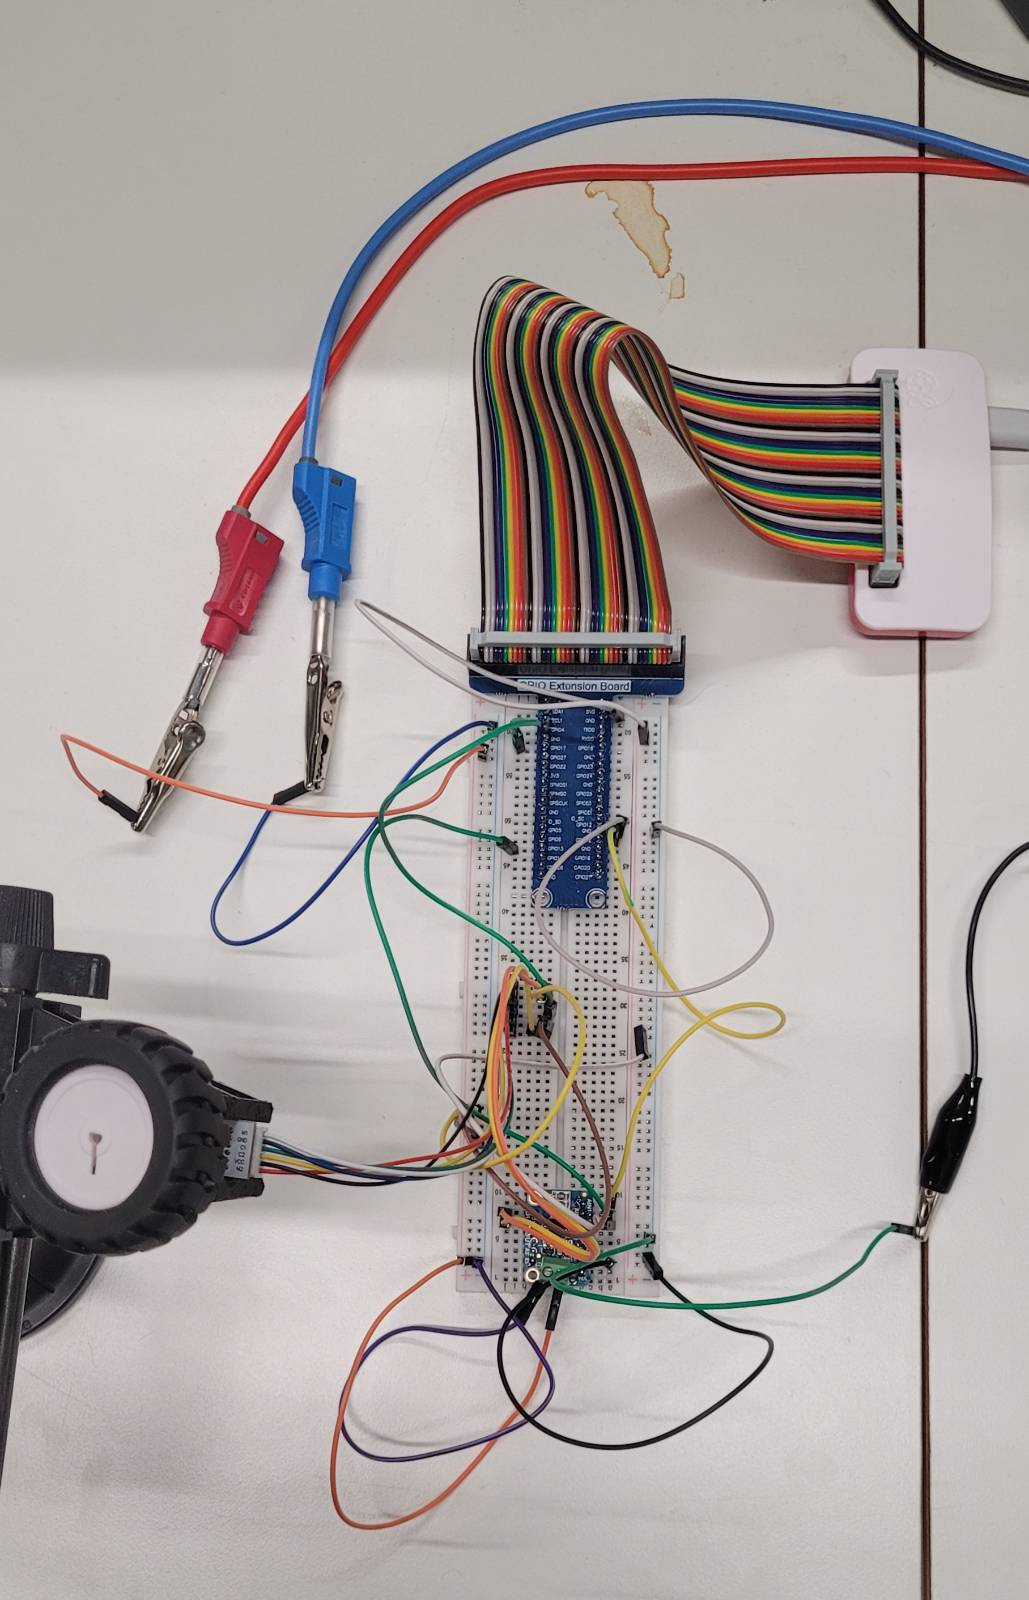
\includegraphics[width=0.55\textwidth]{figures/setup.jpeg}
    \end{center}
    \caption{The assempled system from bottom left to top right: DC motor and tire, motor
    driver, GPIO extension board, Raspberry Pi}\label{fig:assembly}
\end{figure}

The GPIO headers on the RPi were connected to a motor encoder and driver for testing. A
simple P-controller was ported from a previous project and used to test the system, which
was powered by a 7V DC power supply.

\subsection*{Control rate stability}
Time stamps were generated for each step of the control loop.
The control loop had a delay of 5ms and the measured standard deviation was $138.6\mu s$
making the error $\approx 3\%$. The histogram in Figure~\ref{fig:control-hist} provides a
visual representation of the variance, an ideal result would contain only a single bin.
The authors estimate that for critical systems, compensations for timing would be
necessary.
\begin{figure}[h]
    \begin{center}
        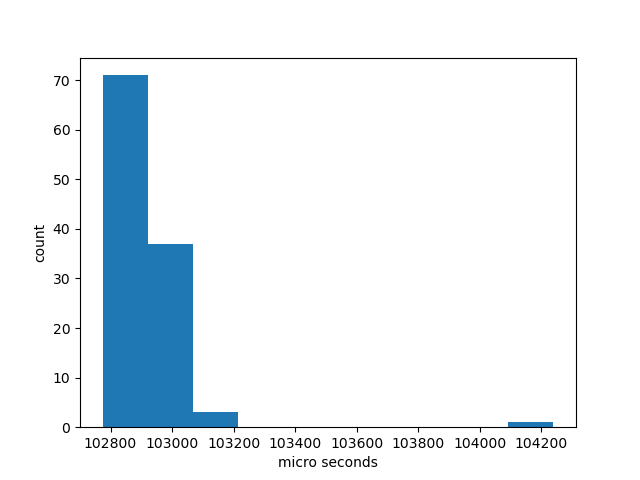
\includegraphics[width=0.65\textwidth]{figures/hist1.png}
    \end{center}
    \caption{Histogram of the time between control steps}\label{fig:control-hist}
\end{figure}

\subsection*{Effects of system-load}
The most notable effects of system-load on the system were the variances in control loop
delay and an increase in delay of stdout.

%\newpage
%\printbibliography

\end{document}
